\documentclass[11pt, letterpaper]{article}

\usepackage[utf8]{inputenc}
\usepackage{epsfig, url}
\usepackage{epstopdf}
\usepackage{tabularx}
\usepackage{graphicx}
\usepackage{datetime}
\usepackage{multirow}
\usepackage{float}
%\usepackage{wrapfig}
\usepackage{amsmath}
\usepackage{amssymb}
\usepackage{geometry} 
\geometry{a4paper}              

\usepackage{titling}
\setlength{\evensidemargin}{0in}
\setlength{\oddsidemargin}{0in}
\setlength{\textwidth}{6.5in}
\setlength{\textheight}{9.0in}
\setlength{\topmargin}{0in}
\setlength{\headheight}{0in}
\setlength{\headsep}{0in}
\setlength{\itemsep}{-\parsep}

\begin{document}

\title{\large Course CS-451: Computational Intelligence\\[0.5cm]
        \bf\Large Assignment 01 - Report}
\author{\large Ali Hamza (ah05084) \\ Haris Karim Ladhani (hl04349) \\ Synclair Samson (ss05901))}
\date{\today}
\makeatletter
    \begin{titlepage}
        \begin{center}
        \vbox{}\vspace{5cm}
            {\@title }\\[3cm] 
            {\@author}\\
            %{Instructor: \bf instructor name}\\
            \vfill 
\includegraphics[scale=0.5]{images/logo.png}\\[1cm]
            {\@date}
        \end{center}
    \end{titlepage}
\makeatother

\newpage

\tableofcontents
\newpage

\section{Travelling Salesman Problem(TSP)}
\subsection{Problem Statement}
The problem involves a traveling salesman who needs to visit several different cities the question is which order to visit the cities to make the shortest possible trip. In which the salesman visits each of the cities once and then returns to the original position. This is an interesting problem cause it can be be applied to  real-world problems and have huge impacts. In this case, we have to find the best route that covers all the cities. \\
Unfortunately a globally optimal path exist for a small number of cities but as the number of cities grows the computation time required grows. To account for these groeing cities and to get an optimized path we are going to use Evolutionary Algorithms in this case, it's going to replicate the nature selection process and get an optimized path with each generation.

\subsection{Chromosome Representation}

\subsection{Fitness Function}
\subsection{Parameters}
The parameters that have been set here are,
\begin{itemize}
    \item Population size: 30
    \item Number of offspring to be produced in each generation :10
    \item No. of generations: 100
    \item Mutation rate: 0.5
    \item No of Iterations: 10
\end{itemize}
\subsection{Results} 
\subsubsection {FPS and Random}
In the case of FPS and Random,

Average Fitness = 

Best Fitness = 
\begin{figure}[H]
    \centering
    
\includegraphics[scale = 0.6]{images/placeHolder.png}
    \caption {Knapsack - FPS \& Random}
    \label {fig:tpsFR}
\end{figure}
\underline{Analysis}
\subsubsection {Binary Tournament and Truncation}
In the case of Binary Tournament and Truncation,

Average Fitness = 

Best Fitness = 
\begin{figure}[h]
    \centering
    
\includegraphics[scale = 0.6]{images/placeHolder.png}
    \caption {Knapsack - Binary Tournament \& Truncation}
    \label {fig:tpsBT}
\end{figure}

\underline{Analysis}

\subsubsection {Truncation and Truncation}
In the case of Truncation and Truncation,

Average Fitness = 

Best Fitness = 
\begin{figure}[H]
    \centering
    
\includegraphics[scale = 0.6]{images/placeHolder.png}
    \caption {Knapsack - Truncation \& Truncation}
    \label {fig:tpsTT}
\end{figure}

\underline{Analysis}
\subsubsection {Random and Random}
In the case of Random and Random,

Average Fitness = 

Best Fitness = 
\begin{figure}[H]
    \centering
    
\includegraphics[scale = 0.6]{images/placeHolder.png}
    \caption {Knapsack - Random \& Random}
    \label {fig:tpsRR}
\end{figure}

\underline{Analysis}
\subsubsection {FPS and Truncation}
In the case of FPS and Truncation,

Average Fitness = 

Best Fitness = 
\begin{figure}[H]
    \centering
    
\includegraphics[scale = 0.6]{images/placeHolder.png}
    \caption {Knapsack - FPS \& Truncation}
    \label {fig:tpsFT}
\end{figure}

\underline{Analysis}
\subsubsection {RBS and Binary Tournament}
In the case of RBS and Binary Tournament,

Average Fitness = 

Best Fitness = 
\begin{figure}[H]
    \centering
    
\includegraphics[scale = 0.6]{images/placeHolder.png}
    \caption {Knapsack - RBS \& Binary Tournament}
    \label {fig:tpsRB}
\end{figure}

\underline{Analysis}
\subsubsection {Random and Truncation}
In the case of Random and Truncation,

Average Fitness = 

Best Fitness = 
\begin{figure}[H]
    \centering
    
\includegraphics[scale = 0.6]{images/placeHolder.png}
    \caption {Knapsack - Random \& Truncation}
    \label {fig:tpsRT}
\end{figure}

\underline{Analysis}
\subsubsection {Truncation and RBS}
In the case of Truncation and RBS,

Average Fitness = 

Best Fitness = 
\begin{figure}[H]
    \centering
    
\includegraphics[scale = 0.6]{images/placeHolder.png}
    \caption {Knapsack - Truncation \& RBS}
    \label {fig:tpsTR}
\end{figure}

\underline{Analysis}
\subsubsection {RBS and Random}
In the case of RBS and Random,

Average Fitness = 

Best Fitness = 
\begin{figure}[H]
    \centering
    
\includegraphics[scale = 0.6]{images/placeHolder.png}
    \caption {Knapsack - RBS \& Random}
    \label {fig:tpsRbR}
\end{figure}

\underline{Analysis}
\subsubsection {Binary Tournament and FPS}
In the case of Binary Tournament and FPS,

Average Fitness = 

Best Fitness = 
\begin{figure}[H]
    \centering
    
\includegraphics[scale = 0.6]{images/placeHolder.png}
    \caption {Knapsack - Binary Tournament \& FPS}
    \label {fig:tpsBF}
\end{figure}

\underline{Analysis}
\subsection {Overall Analysis}

\section{Knapsack Problem}
\subsection{Problem Statement}
In the Knapsack Problem, assume there is a knapsack that is filled with boxes and each box has a 
weight and a value and the objective is to fill the knapsack with the most value without going over 
a specified weight limit. Another good way to imagine this is through the popular aladdin tale. 
Imagiine you are in an aladdin's cave full of treasure but you have one sack and you'd have to fill 
it with.\\
For example, here we have chosen four boxes and each one has a weight that is 5, 4, 7, and 2 
respectively. Now the goal is to put the maximum value of boxes in the sack without going over a 
weight limit i.e. 15 kilograms. A solution for this can be represneted using four bits so for either 0s 
or 1s, each one corresponding to a box. Assuming the first box
won't be included in the knapsack 
the, second one will the third one will and the fourth one won't. Then we can add up the values 
and the weights to see how well this satisfies this problem so the weights are 2 and 1 so that's 3, i.e. 
less than 15 kilograms. We can give this a score on the
value so we can actually return the score 
which is 4 plus 7 which is 11 i.e. the score. In an unsuccessful we can assign 1110 respectively, 
where two boxes are quite heavy so what we know with the limit being 15 if we add 9 and 7 that's 
16 which is above the limit, the solution score is 0. The goal here is to get the best combination of 
boxes so that we can get the most value without being overweight.

\subsection{Chromosome Representation}

\subsection{Fitness Function}

\subsection{Parameters}
The parameters that have been set here are,
\begin{itemize}
    \item Population size: 30
    \item Number of offspring to be produced in each generation :10
    \item No. of generations: 100
    \item Mutation rate: 0.5
    \item No of Iterations: 10
\end{itemize}
\subsection{Results} 
\subsubsection {FPS and Random}
In the case of FPS and Random,

Average Fitness =

Best Fitness = 
\begin{figure}[H]
    \centering
    
\includegraphics[scale = 0.6]{images/placeHolder.png}
    \caption {Knapsack - FPS \& Random}
    \label {fig:kpFR}
\end{figure}
\underline{Analysis}
\subsubsection {Binary Tournament and Truncation}
In the case of Binary Tournament and Truncation,

Average Fitness = 

Best Fitness = 
\begin{figure}[h]
    \centering
    
\includegraphics[scale = 0.6]{images/placeHolder.png}
    \caption {Knapsack - Binary Tournament \& Truncation}
    \label {fig:kpBT}
\end{figure}

\underline{Analysis}

\subsubsection {Truncation and Truncation}
In the case of Truncation and Truncation,

Average Fitness = 

Best Fitness = 
\begin{figure}[H]
    \centering
    
\includegraphics[scale = 0.6]{images/placeHolder.png}
    \caption {Knapsack - Truncation \& Truncation}
    \label {fig:kpTT}
\end{figure}

\underline{Analysis}
\subsubsection {Random and Random}
In the case of Random and Random,

Average Fitness = 

Best Fitness = 
\begin{figure}[H]
    \centering
    
\includegraphics[scale = 0.6]{images/placeHolder.png}
    \caption {Knapsack - Random \& Random}
    \label {fig:kpRR}
\end{figure}

\underline{Analysis}
\subsubsection {FPS and Truncation}
In the case of FPS and Truncation,

Average Fitness = 

Best Fitness = 
\begin{figure}[H]
    \centering
    
\includegraphics[scale = 0.6]{images/placeHolder.png}
    \caption {Knapsack - FPS \& Truncation}
    \label {fig:kpFT}
\end{figure}

\underline{Analysis}
\subsubsection {RBS and Binary Tournament}
In the case of RBS and Binary Tournament,

Average Fitness = 

Best Fitness = 
\begin{figure}[H]
    \centering
    
\includegraphics[scale = 0.6]{images/placeHolder.png}
    \caption {Knapsack - RBS \& Binary Tournament}
    \label {fig:kpRB}
\end{figure}

\underline{Analysis}
\subsubsection {Random and Truncation}
In the case of Random and Truncation,

Average Fitness = 

Best Fitness = 
\begin{figure}[H]
    \centering
    
\includegraphics[scale = 0.6]{images/placeHolder.png}
    \caption {Knapsack - Random \& Truncation}
    \label {fig:kpRT}
\end{figure}

\underline{Analysis}
\subsubsection {Truncation and RBS}
In the case of Truncation and RBS,

Average Fitness = 

Best Fitness = 
\begin{figure}[H]
    \centering
    
\includegraphics[scale = 0.6]{images/placeHolder.png}
    \caption {Knapsack - Truncation \& RBS}
    \label {fig:kpTR}
\end{figure}

\underline{Analysis}
\subsubsection {RBS and Random}
In the case of RBS and Random,

Average Fitness = 

Best Fitness = 
\begin{figure}[H]
    \centering
    
\includegraphics[scale = 0.6]{images/placeHolder.png}
    \caption {Knapsack - RBS \& Random}
    \label {fig:kpRbR}
\end{figure}

\underline{Analysis}
\subsubsection {Binary Tournament and FPS}
In the case of Binary Tournament and FPS,

Average Fitness = 

Best Fitness = 
\begin{figure}[H]
    \centering
    
\includegraphics[scale = 0.6]{images/placeHolder.png}
    \caption {Knapsack - Binary Tournament \& FPS}
    \label {fig:kpBF}
\end{figure}

\underline{Analysis}
\subsection {Overall Analysis}

\section{Graph Coloring}
\subsection {Problem Statement}
In the graph coloring problem, given a graph of vertices and edges that are wanted to color the
nodes in such a way that no two adjacent vertices share a color using the fewest number of colors.
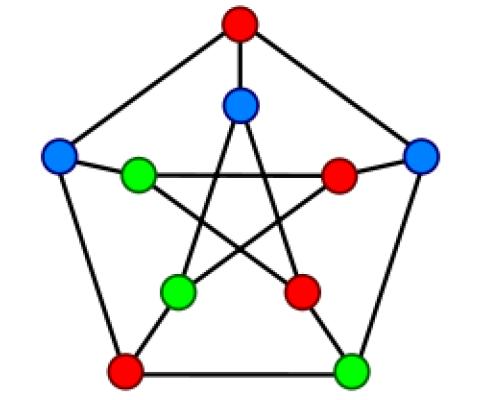
\includegraphics[scale=0.8]{images/graphCol.PNG}\\[1cm]
If we look at this Pentagon star, it can be seen that the two adjacent nodes share a color. For 
example, looking at the top node it can be seen that it only shares an edge with blue and there 
are no Reds attached to it. Then if you look around and all the other nodes throughout this graph 
you'll see that the same property holds true so the problem description is that if we were given a 
graph G and an integer M we want to find if we can color the vertices of a graph with minimum 
colors such that no two adjacent vertices are of same color using at most M colors so this Pentagon 
star problem has ten nodes so it's n value is 10 and M is equal to 3.\\
\subsection {Chromosome Representation}
\subsection {Fitness Function}
\subsection {Parameters}
The parameters that have been set here are,
\begin{itemize}
    \item Population size: 30
    \item Number of offspring to be produced in each generation :10
    \item No. of generations: 100
    \item Mutation rate: 0.5
    \item No of Iterations: 10
\end{itemize}
\subsection {Results} 
\subsubsection {FPS and Random}
In the case of FPS and Random,

Average Fitness = 

Best Fitness = 
\begin{figure}[H]
    \centering
    
\includegraphics[scale = 0.6]{images/placeHolder.png}
    \caption {Knapsack - FPS \& Random}
    \label {fig:gcFR}
\end{figure}
\underline{Analysis}
\subsubsection {Binary Tournament and Truncation}
In the case of Binary Tournament and Truncation,

Average Fitness = 

Best Fitness = 
\begin{figure}[h]
    \centering
    
\includegraphics[scale = 0.6]{images/placeHolder.png}
    \caption {Knapsack - Binary Tournament \& Truncation}
    \label {fig:gcBT}
\end{figure}

\underline{Analysis}

\subsubsection {Truncation and Truncation}
In the case of Truncation and Truncation,

Average Fitness = 

Best Fitness = 
\begin{figure}[H]
    \centering
    
\includegraphics[scale = 0.6]{images/placeHolder.png}
    \caption {Knapsack - Truncation \& Truncation}
    \label {fig:gcTT}
\end{figure}

\underline{Analysis}
\subsubsection {Random and Random}
In the case of Random and Random,

Average Fitness = 

Best Fitness = 
\begin{figure}[H]
    \centering
    
\includegraphics[scale = 0.6]{images/placeHolder.png}
    \caption {Knapsack - Random \& Random}
    \label {fig:gcRR}
\end{figure}

\underline{Analysis}
\subsubsection {FPS and Truncation}
In the case of FPS and Truncation,

Average Fitness = 

Best Fitness = 
\begin{figure}[H]
    \centering
    
\includegraphics[scale = 0.6]{images/placeHolder.png}
    \caption {Knapsack - FPS \& Truncation}
    \label {fig:gcFT}
\end{figure}

\underline{Analysis}
\subsubsection {RBS and Binary Tournament}
In the case of RBS and Binary Tournament,

Average Fitness = 

Best Fitness = 
\begin{figure}[H]
    \centering
    
\includegraphics[scale = 0.6]{images/placeHolder.png}
    \caption {Knapsack - RBS \& Binary Tournament}
    \label {fig:gcRB}
\end{figure}

\underline{Analysis}
\subsubsection {Random and Truncation}
In the case of Random and Truncation,

Average Fitness = 

Best Fitness = 
\begin{figure}[H]
    \centering
    
\includegraphics[scale = 0.6]{images/placeHolder.png}
    \caption {Knapsack - Random \& Truncation}
    \label {fig:gcRT}
\end{figure}

\underline{Analysis}
\subsubsection {Truncation and RBS}
In the case of Truncation and RBS,

Average Fitness = 

Best Fitness = 
\begin{figure}[H]
    \centering
    
\includegraphics[scale = 0.6]{images/placeHolder.png}
    \caption {Knapsack - Truncation \& RBS}
    \label {fig:gcTR}
\end{figure}

\underline{Analysis}
\subsubsection {RBS and Random}
In the case of RBS and Random,

Average Fitness = 

Best Fitness = 
\begin{figure}[H]
    \centering
    
\includegraphics[scale = 0.6]{images/placeHolder.png}
    \caption {Knapsack - RBS \& Random}
    \label {fig:gcRbR}
\end{figure}

\underline{Analysis}
\subsubsection {Binary Tournament and FPS}
In the case of Binary Tournament and FPS,

Average Fitness = 

Best Fitness = 
\begin{figure}[H]
    \centering
    
\includegraphics[scale = 0.6]{images/placeHolder.png}
    \caption {Knapsack - Binary Tournament \& FPS}
    \label {fig:gcBF}
\end{figure}

\underline{Analysis}
\subsection {Overall Analysis}

\end{document}